\documentclass[1p]{elsarticle_modified}
%\bibliographystyle{elsarticle-num}

%\usepackage[colorlinks]{hyperref}
%\usepackage{abbrmath_seonhwa} %\Abb, \Ascr, \Acal ,\Abf, \Afrak
\usepackage{amsfonts}
\usepackage{amssymb}
\usepackage{amsmath}
\usepackage{amsthm}
\usepackage{scalefnt}
\usepackage{amsbsy}
\usepackage{kotex}
\usepackage{caption}
\usepackage{subfig}
\usepackage{color}
\usepackage{graphicx}
\usepackage{xcolor} %% white, black, red, green, blue, cyan, magenta, yellow
\usepackage{float}
\usepackage{setspace}
\usepackage{hyperref}

\usepackage{tikz}
\usetikzlibrary{arrows}

\usepackage{multirow}
\usepackage{array} % fixed length table
\usepackage{hhline}

%%%%%%%%%%%%%%%%%%%%%
\makeatletter
\renewcommand*\env@matrix[1][\arraystretch]{%
	\edef\arraystretch{#1}%
	\hskip -\arraycolsep
	\let\@ifnextchar\new@ifnextchar
	\array{*\c@MaxMatrixCols c}}
\makeatother %https://tex.stackexchange.com/questions/14071/how-can-i-increase-the-line-spacing-in-a-matrix
%%%%%%%%%%%%%%%

\usepackage[normalem]{ulem}

\newcommand{\msout}[1]{\ifmmode\text{\sout{\ensuremath{#1}}}\else\sout{#1}\fi}
%SOURCE: \msout is \stkout macro in https://tex.stackexchange.com/questions/20609/strikeout-in-math-mode

\newcommand{\cancel}[1]{
	\ifmmode
	{\color{red}\msout{#1}}
	\else
	{\color{red}\sout{#1}}
	\fi
}

\newcommand{\add}[1]{
	{\color{blue}\uwave{#1}}
}

\newcommand{\replace}[2]{
	\ifmmode
	{\color{red}\msout{#1}}{\color{blue}\uwave{#2}}
	\else
	{\color{red}\sout{#1}}{\color{blue}\uwave{#2}}
	\fi
}

\newcommand{\Sol}{\mathcal{S}} %segment
\newcommand{\D}{D} %diagram
\newcommand{\A}{\mathcal{A}} %arc


%%%%%%%%%%%%%%%%%%%%%%%%%%%%%5 test

\def\sl{\operatorname{\textup{SL}}(2,\Cbb)}
\def\psl{\operatorname{\textup{PSL}}(2,\Cbb)}
\def\quan{\mkern 1mu \triangleright \mkern 1mu}

\theoremstyle{definition}
\newtheorem{thm}{Theorem}[section]
\newtheorem{prop}[thm]{Proposition}
\newtheorem{lem}[thm]{Lemma}
\newtheorem{ques}[thm]{Question}
\newtheorem{cor}[thm]{Corollary}
\newtheorem{defn}[thm]{Definition}
\newtheorem{exam}[thm]{Example}
\newtheorem{rmk}[thm]{Remark}
\newtheorem{alg}[thm]{Algorithm}

\newcommand{\I}{\sqrt{-1}}
\begin{document}

%\begin{frontmatter}
%
%\title{Boundary parabolic representations of knots up to 8 crossings}
%
%%% Group authors per affiliation:
%\author{Yunhi Cho} 
%\address{Department of Mathematics, University of Seoul, Seoul, Korea}
%\ead{yhcho@uos.ac.kr}
%
%
%\author{Seonhwa Kim} %\fnref{s_kim}}
%\address{Center for Geometry and Physics, Institute for Basic Science, Pohang, 37673, Korea}
%\ead{ryeona17@ibs.re.kr}
%
%\author{Hyuk Kim}
%\address{Department of Mathematical Sciences, Seoul National University, Seoul 08826, Korea}
%\ead{hyukkim@snu.ac.kr}
%
%\author{Seokbeom Yoon}
%\address{Department of Mathematical Sciences, Seoul National University, Seoul, 08826,  Korea}
%\ead{sbyoon15@snu.ac.kr}
%
%\begin{abstract}
%We find all boundary parabolic representation of knots up to 8 crossings.
%
%\end{abstract}
%\begin{keyword}
%    \MSC[2010] 57M25 
%\end{keyword}
%
%\end{frontmatter}

%\linenumbers
%\tableofcontents
%
\newcommand\colored[1]{\textcolor{white}{\rule[-0.35ex]{0.8em}{1.4ex}}\kern-0.8em\color{red} #1}%
%\newcommand\colored[1]{\textcolor{white}{ #1}\kern-2.17ex	\textcolor{white}{ #1}\kern-1.81ex	\textcolor{white}{ #1}\kern-2.15ex\color{red}#1	}

{\Large $\underline{12n_{0803}~(K12n_{0803})}$}

\setlength{\tabcolsep}{10pt}
\renewcommand{\arraystretch}{1.6}
\vspace{1cm}\begin{tabular}{m{100pt}>{\centering\arraybackslash}m{274pt}}
\multirow{5}{120pt}{
	\centering
	\includegraphics[width=112pt]{../../../GIT/diagram.site/Diagrams/png/2892_12n_0803.png}\\
\ \ \ A knot diagram\footnotemark}&
\allowdisplaybreaks
\textbf{Linearized knot diagam} \\
\cline{2-2}
 &
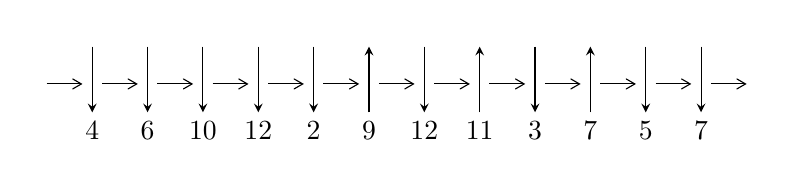
\begin{tikzpicture}[x=20pt, y=17pt]
	% nodes
	\node (C0) at (0, 0) {};
	\node (C1) at (1, 0) {};
	\node (C1U) at (1, +1) {};
	\node (C1D) at (1, -1) {4};

	\node (C2) at (2, 0) {};
	\node (C2U) at (2, +1) {};
	\node (C2D) at (2, -1) {6};

	\node (C3) at (3, 0) {};
	\node (C3U) at (3, +1) {};
	\node (C3D) at (3, -1) {10};

	\node (C4) at (4, 0) {};
	\node (C4U) at (4, +1) {};
	\node (C4D) at (4, -1) {12};

	\node (C5) at (5, 0) {};
	\node (C5U) at (5, +1) {};
	\node (C5D) at (5, -1) {2};

	\node (C6) at (6, 0) {};
	\node (C6U) at (6, +1) {};
	\node (C6D) at (6, -1) {9};

	\node (C7) at (7, 0) {};
	\node (C7U) at (7, +1) {};
	\node (C7D) at (7, -1) {12};

	\node (C8) at (8, 0) {};
	\node (C8U) at (8, +1) {};
	\node (C8D) at (8, -1) {11};

	\node (C9) at (9, 0) {};
	\node (C9U) at (9, +1) {};
	\node (C9D) at (9, -1) {3};

	\node (C10) at (10, 0) {};
	\node (C10U) at (10, +1) {};
	\node (C10D) at (10, -1) {7};

	\node (C11) at (11, 0) {};
	\node (C11U) at (11, +1) {};
	\node (C11D) at (11, -1) {5};

	\node (C12) at (12, 0) {};
	\node (C12U) at (12, +1) {};
	\node (C12D) at (12, -1) {7};
	\node (C13) at (13, 0) {};

	% arrows
	\draw[->,>={angle 60}]
	(C0) edge (C1) (C1) edge (C2) (C2) edge (C3) (C3) edge (C4) (C4) edge (C5) (C5) edge (C6) (C6) edge (C7) (C7) edge (C8) (C8) edge (C9) (C9) edge (C10) (C10) edge (C11) (C11) edge (C12) (C12) edge (C13) ;	\draw[->,>=stealth]
	(C1U) edge (C1D) (C2U) edge (C2D) (C3U) edge (C3D) (C4U) edge (C4D) (C5U) edge (C5D) (C6D) edge (C6U) (C7U) edge (C7D) (C8D) edge (C8U) (C9U) edge (C9D) (C10D) edge (C10U) (C11U) edge (C11D) (C12U) edge (C12D) ;
	\end{tikzpicture} \\
\hhline{~~} \\& 
\textbf{Solving Sequence} \\ \cline{2-2} 
 &
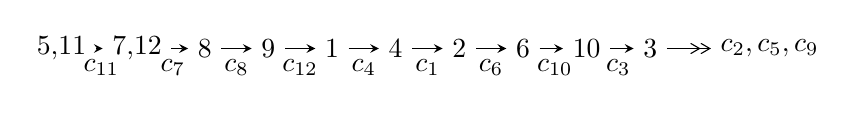
\begin{tikzpicture}[x=23pt, y=7pt]
	% node
	\node (A0) at (-1/8, 0) {5,11};
	\node (A1) at (17/16, 0) {7,12};
	\node (A2) at (17/8, 0) {8};
	\node (A3) at (25/8, 0) {9};
	\node (A4) at (33/8, 0) {1};
	\node (A5) at (41/8, 0) {4};
	\node (A6) at (49/8, 0) {2};
	\node (A7) at (57/8, 0) {6};
	\node (A8) at (65/8, 0) {10};
	\node (A9) at (73/8, 0) {3};
	\node (C1) at (1/2, -1) {$c_{11}$};
	\node (C2) at (13/8, -1) {$c_{7}$};
	\node (C3) at (21/8, -1) {$c_{8}$};
	\node (C4) at (29/8, -1) {$c_{12}$};
	\node (C5) at (37/8, -1) {$c_{4}$};
	\node (C6) at (45/8, -1) {$c_{1}$};
	\node (C7) at (53/8, -1) {$c_{6}$};
	\node (C8) at (61/8, -1) {$c_{10}$};
	\node (C9) at (69/8, -1) {$c_{3}$};
	\node (A10) at (11, 0) {$c_{2},c_{5},c_{9}$};

	% edge
	\draw[->,>=stealth]	
	(A0) edge (A1) (A1) edge (A2) (A2) edge (A3) (A3) edge (A4) (A4) edge (A5) (A5) edge (A6) (A6) edge (A7) (A7) edge (A8) (A8) edge (A9) ;
	\draw[->>,>={angle 60}]	
	(A9) edge (A10);
\end{tikzpicture} \\ 

\end{tabular} \\

\footnotetext{
The image of knot diagram is generated by the software ``\textbf{Draw programme}" developed by Andrew Bartholomew(\url{http://www.layer8.co.uk/maths/draw/index.htm\#Running-draw}), where we modified some parts for our purpose(\url{https://github.com/CATsTAILs/LinksPainter}).
}\phantom \\ \newline 
\centering \textbf{Ideals for irreducible components\footnotemark of $X_{\text{par}}$} 
 
\begin{align*}
I^u_{1}&=\langle 
-20967 u^{23}+422302 u^{22}+\cdots+119758 b+1936892,\\
\phantom{I^u_{1}}&\phantom{= \langle  }333347 u^{23}+3142111 u^{22}+\cdots+119758 a+1463683,\;u^{24}+8 u^{23}+\cdots+34 u+4\rangle \\
I^u_{2}&=\langle 
20658081418 u^{25} a+11852435996417 u^{25}+\cdots-20658081418 a+1592388657005,\\
\phantom{I^u_{2}}&\phantom{= \langle  }-34939904896 u^{25} a+44997972497 u^{25}+\cdots+97240087620 a+132117488383,\\
\phantom{I^u_{2}}&\phantom{= \langle  }u^{26}-3 u^{25}+\cdots+6 u^2+1\rangle \\
I^u_{3}&=\langle 
- u^{11}-2 u^{10}-5 u^9-5 u^8-7 u^7-2 u^6-2 u^5+4 u^4+u^3+3 u^2+b- u+1,\\
\phantom{I^u_{3}}&\phantom{= \langle  }- u^{11}-4 u^{10}-11 u^9-20 u^8-30 u^7-34 u^6-32 u^5-23 u^4-13 u^3-6 u^2+a-3 u-3,\\
\phantom{I^u_{3}}&\phantom{= \langle  }u^{12}+3 u^{11}+8 u^{10}+13 u^9+20 u^8+21 u^7+22 u^6+15 u^5+12 u^4+5 u^3+5 u^2+u+1\rangle \\
I^u_{4}&=\langle 
u^5 a+3 u^5+3 u^3 a-5 u^4-4 u^2 a+9 u^3+4 a u-7 u^2+5 b- a+7 u+2,\\
\phantom{I^u_{4}}&\phantom{= \langle  }u^4 a+2 u^5-2 u^3 a-3 u^4+3 u^2 a+6 u^3+a^2-3 a u-6 u^2+2 a+5 u,\;u^6- u^5+3 u^4-2 u^3+3 u^2+1\rangle \\
\\
\end{align*}
\raggedright * 4 irreducible components of $\dim_{\mathbb{C}}=0$, with total 100 representations.\\
\footnotetext{All coefficients of polynomials are rational numbers. But the coefficients are sometimes approximated in decimal forms when there is not enough margin.}
\newpage
\renewcommand{\arraystretch}{1}
\centering \section*{I. $I^u_{1}= \langle -2.10\times10^{4} u^{23}+4.22\times10^{5} u^{22}+\cdots+1.20\times10^{5} b+1.94\times10^{6},\;3.33\times10^{5} u^{23}+3.14\times10^{6} u^{22}+\cdots+1.20\times10^{5} a+1.46\times10^{6},\;u^{24}+8 u^{23}+\cdots+34 u+4 \rangle$}
\flushleft \textbf{(i) Arc colorings}\\
\begin{tabular}{m{7pt} m{180pt} m{7pt} m{180pt} }
\flushright $a_{5}=$&$\begin{pmatrix}0\\u\end{pmatrix}$ \\
\flushright $a_{11}=$&$\begin{pmatrix}1\\0\end{pmatrix}$ \\
\flushright $a_{7}=$&$\begin{pmatrix}-2.78351 u^{23}-26.2372 u^{22}+\cdots-145.274 u-12.2220\\0.175078 u^{23}-3.52629 u^{22}+\cdots-106.512 u-16.1734\end{pmatrix}$ \\
\flushright $a_{12}=$&$\begin{pmatrix}1\\u^2\end{pmatrix}$ \\
\flushright $a_{8}=$&$\begin{pmatrix}8.01248 u^{23}+53.3038 u^{22}+\cdots+107.322 u+19.8279\\-3.96913 u^{23}-20.7820 u^{22}+\cdots+82.4172 u+11.1340\end{pmatrix}$ \\
\flushright $a_{9}=$&$\begin{pmatrix}4.04335 u^{23}+32.5218 u^{22}+\cdots+189.739 u+30.9619\\-3.96913 u^{23}-20.7820 u^{22}+\cdots+82.4172 u+11.1340\end{pmatrix}$ \\
\flushright $a_{1}=$&$\begin{pmatrix}8.35351 u^{23}+54.4948 u^{22}+\cdots-21.7233 u-14.7332\\7.47725 u^{23}+53.9440 u^{22}+\cdots+159.286 u+21.2134\end{pmatrix}$ \\
\flushright $a_{4}=$&$\begin{pmatrix}u\\u^3+u\end{pmatrix}$ \\
\flushright $a_{2}=$&$\begin{pmatrix}-5.30335 u^{23}-34.9495 u^{22}+\cdots-94.8437 u-20.0274\\-18.2073 u^{23}-140.297 u^{22}+\cdots-532.766 u-63.3231\end{pmatrix}$ \\
\flushright $a_{6}=$&$\begin{pmatrix}0.615082 u^{23}+4.89107 u^{22}+\cdots+95.0362 u+24.8300\\-11.8092 u^{23}-78.8511 u^{22}+\cdots-94.1786 u-11.2650\end{pmatrix}$ \\
\flushright $a_{10}=$&$\begin{pmatrix}2.17390 u^{23}+18.9945 u^{22}+\cdots+64.4428 u+1.18601\\0.810526 u^{23}+8.98427 u^{22}+\cdots+96.0801 u+14.8004\end{pmatrix}$ \\
\flushright $a_{3}=$&$\begin{pmatrix}-3.08556 u^{23}-21.2898 u^{22}+\cdots-85.1959 u-19.1276\\-4.41553 u^{23}-33.4970 u^{22}+\cdots-93.2357 u-7.87618\end{pmatrix}$\\&\end{tabular}
\flushleft \textbf{(ii) Obstruction class $= -1$}\\~\\
\flushleft \textbf{(iii) Cusp Shapes $= \frac{248067}{59879} u^{23}+\frac{1208199}{59879} u^{22}+\cdots-\frac{6272226}{59879} u-\frac{1406970}{59879}$}\\~\\
\newpage\renewcommand{\arraystretch}{1}
\flushleft \textbf{(iv) u-Polynomials at the component}\newline \\
\begin{tabular}{m{50pt}|m{274pt}}
Crossings & \hspace{64pt}u-Polynomials at each crossing \\
\hline $$\begin{aligned}c_{1}\end{aligned}$$&$\begin{aligned}
&u^{24}-29 u^{23}+\cdots+8704 u-1024
\end{aligned}$\\
\hline $$\begin{aligned}c_{2},c_{3},c_{5}\\c_{9}\end{aligned}$$&$\begin{aligned}
&u^{24}-12 u^{22}+\cdots+4 u-1
\end{aligned}$\\
\hline $$\begin{aligned}c_{4},c_{11}\end{aligned}$$&$\begin{aligned}
&u^{24}+8 u^{23}+\cdots+34 u+4
\end{aligned}$\\
\hline $$\begin{aligned}c_{6}\end{aligned}$$&$\begin{aligned}
&u^{24}+19 u^{23}+\cdots+480 u+16
\end{aligned}$\\
\hline $$\begin{aligned}c_{7},c_{12}\end{aligned}$$&$\begin{aligned}
&u^{24}+u^{23}+\cdots+2 u+1
\end{aligned}$\\
\hline $$\begin{aligned}c_{8}\end{aligned}$$&$\begin{aligned}
&u^{24}+u^{23}+\cdots+241 u+38
\end{aligned}$\\
\hline $$\begin{aligned}c_{10}\end{aligned}$$&$\begin{aligned}
&u^{24}+2 u^{23}+\cdots+66 u+7
\end{aligned}$\\
\hline
\end{tabular}\\~\\
\newpage\renewcommand{\arraystretch}{1}
\flushleft \textbf{(v) Riley Polynomials at the component}\newline \\
\begin{tabular}{m{50pt}|m{274pt}}
Crossings & \hspace{64pt}Riley Polynomials at each crossing \\
\hline $$\begin{aligned}c_{1}\end{aligned}$$&$\begin{aligned}
&y^{24}-19 y^{23}+\cdots+52690944 y+1048576
\end{aligned}$\\
\hline $$\begin{aligned}c_{2},c_{3},c_{5}\\c_{9}\end{aligned}$$&$\begin{aligned}
&y^{24}-24 y^{23}+\cdots-2 y+1
\end{aligned}$\\
\hline $$\begin{aligned}c_{4},c_{11}\end{aligned}$$&$\begin{aligned}
&y^{24}+8 y^{23}+\cdots-268 y+16
\end{aligned}$\\
\hline $$\begin{aligned}c_{6}\end{aligned}$$&$\begin{aligned}
&y^{24}-5 y^{23}+\cdots-88736 y+256
\end{aligned}$\\
\hline $$\begin{aligned}c_{7},c_{12}\end{aligned}$$&$\begin{aligned}
&y^{24}-37 y^{23}+\cdots-26 y+1
\end{aligned}$\\
\hline $$\begin{aligned}c_{8}\end{aligned}$$&$\begin{aligned}
&y^{24}+27 y^{23}+\cdots-37637 y+1444
\end{aligned}$\\
\hline $$\begin{aligned}c_{10}\end{aligned}$$&$\begin{aligned}
&y^{24}+14 y^{23}+\cdots-548 y+49
\end{aligned}$\\
\hline
\end{tabular}\\~\\
\newpage\flushleft \textbf{(vi) Complex Volumes and Cusp Shapes}
$$\begin{array}{c|c|c}  
\text{Solutions to }I^u_{1}& \I (\text{vol} + \sqrt{-1}CS) & \text{Cusp shape}\\
 \hline 
\begin{aligned}
u &= \phantom{-}0.328897 + 0.963555 I \\
a &= \phantom{-}0.910844 + 0.484743 I \\
b &= -0.766113 + 0.751089 I\end{aligned}
 & -4.13392 - 1.43705 I & -8.07864 + 3.13596 I \\ \hline\begin{aligned}
u &= \phantom{-}0.328897 - 0.963555 I \\
a &= \phantom{-}0.910844 - 0.484743 I \\
b &= -0.766113 - 0.751089 I\end{aligned}
 & -4.13392 + 1.43705 I & -8.07864 - 3.13596 I \\ \hline\begin{aligned}
u &= \phantom{-}0.939855 + 0.071846 I \\
a &= -0.404510 + 0.906423 I \\
b &= -0.691190 + 1.173450 I\end{aligned}
 & -7.64599 + 2.14568 I & -13.26685 - 1.01150 I \\ \hline\begin{aligned}
u &= \phantom{-}0.939855 - 0.071846 I \\
a &= -0.404510 - 0.906423 I \\
b &= -0.691190 - 1.173450 I\end{aligned}
 & -7.64599 - 2.14568 I & -13.26685 + 1.01150 I \\ \hline\begin{aligned}
u &= -0.746626 + 0.871724 I \\
a &= -1.08140 + 1.18930 I \\
b &= -0.239897 + 0.846639 I\end{aligned}
 & -10.39910 + 0.71995 I & -14.8370 + 0.2681 I \\ \hline\begin{aligned}
u &= -0.746626 - 0.871724 I \\
a &= -1.08140 - 1.18930 I \\
b &= -0.239897 - 0.846639 I\end{aligned}
 & -10.39910 - 0.71995 I & -14.8370 - 0.2681 I \\ \hline\begin{aligned}
u &= -0.778661 + 0.901540 I \\
a &= \phantom{-}0.34330 - 1.73842 I \\
b &= -0.437819 - 1.055850 I\end{aligned}
 & -10.32800 + 5.07117 I & -14.4995 - 5.6581 I \\ \hline\begin{aligned}
u &= -0.778661 - 0.901540 I \\
a &= \phantom{-}0.34330 + 1.73842 I \\
b &= -0.437819 + 1.055850 I\end{aligned}
 & -10.32800 - 5.07117 I & -14.4995 + 5.6581 I \\ \hline\begin{aligned}
u &= -0.973000 + 0.794755 I \\
a &= -0.434212 + 0.833754 I \\
b &= -0.310872 + 1.186700 I\end{aligned}
 & -3.59091 + 0.70472 I & -5.59047 + 0.17704 I \\ \hline\begin{aligned}
u &= -0.973000 - 0.794755 I \\
a &= -0.434212 - 0.833754 I \\
b &= -0.310872 - 1.186700 I\end{aligned}
 & -3.59091 - 0.70472 I & -5.59047 - 0.17704 I\\
 \hline 
 \end{array}$$\newpage$$\begin{array}{c|c|c}  
\text{Solutions to }I^u_{1}& \I (\text{vol} + \sqrt{-1}CS) & \text{Cusp shape}\\
 \hline 
\begin{aligned}
u &= \phantom{-}0.306537 + 0.623051 I \\
a &= -0.22994 - 1.50030 I \\
b &= \phantom{-}1.000310 - 0.279529 I\end{aligned}
 & \phantom{-}1.86738 - 1.10899 I & \phantom{-}2.50012 + 5.93987 I \\ \hline\begin{aligned}
u &= \phantom{-}0.306537 - 0.623051 I \\
a &= -0.22994 + 1.50030 I \\
b &= \phantom{-}1.000310 + 0.279529 I\end{aligned}
 & \phantom{-}1.86738 + 1.10899 I & \phantom{-}2.50012 - 5.93987 I \\ \hline\begin{aligned}
u &= -0.143155 + 1.299360 I \\
a &= \phantom{-}0.335755 - 0.304928 I \\
b &= -0.292872 + 0.366676 I\end{aligned}
 & \phantom{-}3.50852 + 1.95287 I & -10.85589 - 6.35743 I \\ \hline\begin{aligned}
u &= -0.143155 - 1.299360 I \\
a &= \phantom{-}0.335755 + 0.304928 I \\
b &= -0.292872 - 0.366676 I\end{aligned}
 & \phantom{-}3.50852 - 1.95287 I & -10.85589 + 6.35743 I \\ \hline\begin{aligned}
u &= -0.867739 + 1.076530 I \\
a &= \phantom{-}0.617487 - 1.083160 I \\
b &= -0.735051 - 1.110270 I\end{aligned}
 & -2.71430 + 6.07423 I & -4.21792 - 5.12279 I \\ \hline\begin{aligned}
u &= -0.867739 - 1.076530 I \\
a &= \phantom{-}0.617487 + 1.083160 I \\
b &= -0.735051 + 1.110270 I\end{aligned}
 & -2.71430 - 6.07423 I & -4.21792 + 5.12279 I \\ \hline\begin{aligned}
u &= -1.124970 + 0.818587 I \\
a &= \phantom{-}0.772531 - 0.690664 I \\
b &= \phantom{-}0.92580 - 1.72837 I\end{aligned}
 & -13.8026 - 8.9954 I & -11.74034 + 3.92566 I \\ \hline\begin{aligned}
u &= -1.124970 - 0.818587 I \\
a &= \phantom{-}0.772531 + 0.690664 I \\
b &= \phantom{-}0.92580 + 1.72837 I\end{aligned}
 & -13.8026 + 8.9954 I & -11.74034 - 3.92566 I \\ \hline\begin{aligned}
u &= \phantom{-}0.31884 + 1.40808 I \\
a &= -0.445331 + 0.435914 I \\
b &= -0.006177 - 1.106850 I\end{aligned}
 & -2.95010 - 7.04627 I & -12.05914 + 3.57746 I \\ \hline\begin{aligned}
u &= \phantom{-}0.31884 - 1.40808 I \\
a &= -0.445331 - 0.435914 I \\
b &= -0.006177 + 1.106850 I\end{aligned}
 & -2.95010 + 7.04627 I & -12.05914 - 3.57746 I\\
 \hline 
 \end{array}$$\newpage$$\begin{array}{c|c|c}  
\text{Solutions to }I^u_{1}& \I (\text{vol} + \sqrt{-1}CS) & \text{Cusp shape}\\
 \hline 
\begin{aligned}
u &= -0.91822 + 1.13051 I \\
a &= -0.71706 + 1.35307 I \\
b &= \phantom{-}1.25897 + 1.53619 I\end{aligned}
 & -12.7586 + 16.3728 I & -10.30097 - 7.90933 I \\ \hline\begin{aligned}
u &= -0.91822 - 1.13051 I \\
a &= -0.71706 - 1.35307 I \\
b &= \phantom{-}1.25897 - 1.53619 I\end{aligned}
 & -12.7586 - 16.3728 I & -10.30097 + 7.90933 I \\ \hline\begin{aligned}
u &= -0.429045\phantom{ +0.000000I} \\
a &= \phantom{-}0.412338\phantom{ +0.000000I} \\
b &= -0.233949\phantom{ +0.000000I}\end{aligned}
 & -0.678253\phantom{ +0.000000I} & -14.6600\phantom{ +0.000000I} \\ \hline\begin{aligned}
u &= -0.254478\phantom{ +0.000000I} \\
a &= \phantom{-}4.25274\phantom{ +0.000000I} \\
b &= -1.17623\phantom{ +0.000000I}\end{aligned}
 & -8.31112\phantom{ +0.000000I} & -10.4470\phantom{ +0.000000I}\\
 \hline 
 \end{array}$$\newpage\newpage\renewcommand{\arraystretch}{1}
\centering \section*{II. $I^u_{2}= \langle 2.07\times10^{10} a u^{25}+1.19\times10^{13} u^{25}+\cdots-2.07\times10^{10} a+1.59\times10^{12},\;-3.49\times10^{10} a u^{25}+4.50\times10^{10} u^{25}+\cdots+9.72\times10^{10} a+1.32\times10^{11},\;u^{26}-3 u^{25}+\cdots+6 u^2+1 \rangle$}
\flushleft \textbf{(i) Arc colorings}\\
\begin{tabular}{m{7pt} m{180pt} m{7pt} m{180pt} }
\flushright $a_{5}=$&$\begin{pmatrix}0\\u\end{pmatrix}$ \\
\flushright $a_{11}=$&$\begin{pmatrix}1\\0\end{pmatrix}$ \\
\flushright $a_{7}=$&$\begin{pmatrix}a\\-0.00257732 a u^{25}-1.47872 u^{25}+\cdots+0.00257732 a-0.198668\end{pmatrix}$ \\
\flushright $a_{12}=$&$\begin{pmatrix}1\\u^2\end{pmatrix}$ \\
\flushright $a_{8}=$&$\begin{pmatrix}0.00257732 a u^{25}+1.47872 u^{25}+\cdots+0.997423 a+0.198668\\-2.02614 u^{25}+4.93564 u^{24}+\cdots-2.35356 u-0.845672\end{pmatrix}$ \\
\flushright $a_{9}=$&$\begin{pmatrix}0.00257732 a u^{25}-0.547418 u^{25}+\cdots+0.997423 a-0.647004\\-2.02614 u^{25}+4.93564 u^{24}+\cdots-2.35356 u-0.845672\end{pmatrix}$ \\
\flushright $a_{1}=$&$\begin{pmatrix}0.647004 a u^{25}-0.0669635 u^{25}+\cdots-1.47872 a-0.0221495\\0.151236 a u^{25}-0.930203 u^{25}+\cdots-0.931302 a+1.59748\end{pmatrix}$ \\
\flushright $a_{4}=$&$\begin{pmatrix}u\\u^3+u\end{pmatrix}$ \\
\flushright $a_{2}=$&$\begin{pmatrix}0.647004 a u^{25}+0.0150165 u^{25}+\cdots-1.47872 a-0.0947257\\0.151236 a u^{25}-1.17846 u^{25}+\cdots-0.931302 a+1.70643\end{pmatrix}$ \\
\flushright $a_{6}=$&$\begin{pmatrix}0.198084 a u^{25}-0.0227350 u^{25}+\cdots+0.518890 a+1.13733\\0.349848 a u^{25}-0.457338 u^{25}+\cdots+0.00892927 a+1.26221\end{pmatrix}$ \\
\flushright $a_{10}=$&$\begin{pmatrix}-0.495767 a u^{25}+0.647416 u^{25}+\cdots+0.547418 a+0.138652\\0.304060 a u^{25}-0.977539 u^{25}+\cdots-0.923265 a+1.73692\end{pmatrix}$ \\
\flushright $a_{3}=$&$\begin{pmatrix}0.00515464 a u^{25}+0.448336 u^{25}+\cdots+0.994845 a-0.603879\\-0.187775 a u^{25}+1.12169 u^{25}+\cdots+0.470801 a-3.06193\end{pmatrix}$\\&\end{tabular}
\flushleft \textbf{(ii) Obstruction class $= -1$}\\~\\
\flushleft \textbf{(iii) Cusp Shapes $= -\frac{66478862888}{10329040709} u^{25}+\frac{217968421278}{10329040709} u^{24}+\cdots-\frac{74797871360}{10329040709} u+\frac{51959996001}{10329040709}$}\\~\\
\newpage\renewcommand{\arraystretch}{1}
\flushleft \textbf{(iv) u-Polynomials at the component}\newline \\
\begin{tabular}{m{50pt}|m{274pt}}
Crossings & \hspace{64pt}u-Polynomials at each crossing \\
\hline $$\begin{aligned}c_{1}\end{aligned}$$&$\begin{aligned}
&(u^{26}+7 u^{25}+\cdots+104 u+1)^{2}
\end{aligned}$\\
\hline $$\begin{aligned}c_{2},c_{3},c_{5}\\c_{9}\end{aligned}$$&$\begin{aligned}
&u^{52}+u^{51}+\cdots+9 u+1
\end{aligned}$\\
\hline $$\begin{aligned}c_{4},c_{11}\end{aligned}$$&$\begin{aligned}
&(u^{26}-3 u^{25}+\cdots+6 u^2+1)^{2}
\end{aligned}$\\
\hline $$\begin{aligned}c_{6}\end{aligned}$$&$\begin{aligned}
&(u^{26}-5 u^{25}+\cdots-114 u+31)^{2}
\end{aligned}$\\
\hline $$\begin{aligned}c_{7},c_{12}\end{aligned}$$&$\begin{aligned}
&u^{52}+2 u^{51}+\cdots+26027 u+12491
\end{aligned}$\\
\hline $$\begin{aligned}c_{8}\end{aligned}$$&$\begin{aligned}
&u^{52}+4 u^{51}+\cdots-283294 u+74171
\end{aligned}$\\
\hline $$\begin{aligned}c_{10}\end{aligned}$$&$\begin{aligned}
&u^{52}-5 u^{51}+\cdots-453512 u+54833
\end{aligned}$\\
\hline
\end{tabular}\\~\\
\newpage\renewcommand{\arraystretch}{1}
\flushleft \textbf{(v) Riley Polynomials at the component}\newline \\
\begin{tabular}{m{50pt}|m{274pt}}
Crossings & \hspace{64pt}Riley Polynomials at each crossing \\
\hline $$\begin{aligned}c_{1}\end{aligned}$$&$\begin{aligned}
&(y^{26}-31 y^{25}+\cdots-4608 y+1)^{2}
\end{aligned}$\\
\hline $$\begin{aligned}c_{2},c_{3},c_{5}\\c_{9}\end{aligned}$$&$\begin{aligned}
&y^{52}-37 y^{51}+\cdots-13 y+1
\end{aligned}$\\
\hline $$\begin{aligned}c_{4},c_{11}\end{aligned}$$&$\begin{aligned}
&(y^{26}+7 y^{25}+\cdots+12 y+1)^{2}
\end{aligned}$\\
\hline $$\begin{aligned}c_{6}\end{aligned}$$&$\begin{aligned}
&(y^{26}+17 y^{25}+\cdots+11618 y+961)^{2}
\end{aligned}$\\
\hline $$\begin{aligned}c_{7},c_{12}\end{aligned}$$&$\begin{aligned}
&y^{52}-42 y^{51}+\cdots-2616007929 y+156025081
\end{aligned}$\\
\hline $$\begin{aligned}c_{8}\end{aligned}$$&$\begin{aligned}
&y^{52}+38 y^{51}+\cdots+245786133074 y+5501337241
\end{aligned}$\\
\hline $$\begin{aligned}c_{10}\end{aligned}$$&$\begin{aligned}
&y^{52}+27 y^{51}+\cdots-49791469092 y+3006657889
\end{aligned}$\\
\hline
\end{tabular}\\~\\
\newpage\flushleft \textbf{(vi) Complex Volumes and Cusp Shapes}
$$\begin{array}{c|c|c}  
\text{Solutions to }I^u_{2}& \I (\text{vol} + \sqrt{-1}CS) & \text{Cusp shape}\\
 \hline 
\begin{aligned}
u &= \phantom{-}0.131355 + 0.894729 I \\
a &= \phantom{-}0.451077 - 0.150456 I \\
b &= -0.998984 - 0.827868 I\end{aligned}
 & -3.87482 + 4.61379 I & -6.13572 - 1.30037 I \\ \hline\begin{aligned}
u &= \phantom{-}0.131355 + 0.894729 I \\
a &= -1.91778 + 1.70748 I \\
b &= \phantom{-}0.443117 - 0.656912 I\end{aligned}
 & -3.87482 + 4.61379 I & -6.13572 - 1.30037 I \\ \hline\begin{aligned}
u &= \phantom{-}0.131355 - 0.894729 I \\
a &= \phantom{-}0.451077 + 0.150456 I \\
b &= -0.998984 + 0.827868 I\end{aligned}
 & -3.87482 - 4.61379 I & -6.13572 + 1.30037 I \\ \hline\begin{aligned}
u &= \phantom{-}0.131355 - 0.894729 I \\
a &= -1.91778 - 1.70748 I \\
b &= \phantom{-}0.443117 + 0.656912 I\end{aligned}
 & -3.87482 - 4.61379 I & -6.13572 + 1.30037 I \\ \hline\begin{aligned}
u &= -0.398785 + 0.702857 I \\
a &= -0.02931 + 1.44387 I \\
b &= \phantom{-}0.514475 + 0.867181 I\end{aligned}
 & -0.83541 + 4.01832 I & -5.46093 - 8.67700 I \\ \hline\begin{aligned}
u &= -0.398785 + 0.702857 I \\
a &= \phantom{-}1.43554 - 0.33694 I \\
b &= -0.856528 - 0.541924 I\end{aligned}
 & -0.83541 + 4.01832 I & -5.46093 - 8.67700 I \\ \hline\begin{aligned}
u &= -0.398785 - 0.702857 I \\
a &= -0.02931 - 1.44387 I \\
b &= \phantom{-}0.514475 - 0.867181 I\end{aligned}
 & -0.83541 - 4.01832 I & -5.46093 + 8.67700 I \\ \hline\begin{aligned}
u &= -0.398785 - 0.702857 I \\
a &= \phantom{-}1.43554 + 0.33694 I \\
b &= -0.856528 + 0.541924 I\end{aligned}
 & -0.83541 - 4.01832 I & -5.46093 + 8.67700 I \\ \hline\begin{aligned}
u &= \phantom{-}0.874874 + 0.827469 I \\
a &= -0.419640 - 0.908306 I \\
b &= -0.485265 - 1.142940 I\end{aligned}
 & -6.97798 - 4.77378 I & -9.07326 + 3.55688 I \\ \hline\begin{aligned}
u &= \phantom{-}0.874874 + 0.827469 I \\
a &= \phantom{-}0.21817 + 1.45332 I \\
b &= -0.539013 + 1.157240 I\end{aligned}
 & -6.97798 - 4.77378 I & -9.07326 + 3.55688 I\\
 \hline 
 \end{array}$$\newpage$$\begin{array}{c|c|c}  
\text{Solutions to }I^u_{2}& \I (\text{vol} + \sqrt{-1}CS) & \text{Cusp shape}\\
 \hline 
\begin{aligned}
u &= \phantom{-}0.874874 - 0.827469 I \\
a &= -0.419640 + 0.908306 I \\
b &= -0.485265 + 1.142940 I\end{aligned}
 & -6.97798 + 4.77378 I & -9.07326 - 3.55688 I \\ \hline\begin{aligned}
u &= \phantom{-}0.874874 - 0.827469 I \\
a &= \phantom{-}0.21817 - 1.45332 I \\
b &= -0.539013 - 1.157240 I\end{aligned}
 & -6.97798 + 4.77378 I & -9.07326 - 3.55688 I \\ \hline\begin{aligned}
u &= \phantom{-}0.509450 + 0.561310 I \\
a &= -0.40989 + 1.82180 I \\
b &= -0.36665 + 1.55437 I\end{aligned}
 & -5.31435 - 7.28077 I & -10.22138 + 9.25036 I \\ \hline\begin{aligned}
u &= \phantom{-}0.509450 + 0.561310 I \\
a &= \phantom{-}1.92175 + 0.40718 I \\
b &= -0.842568 + 0.445418 I\end{aligned}
 & -5.31435 - 7.28077 I & -10.22138 + 9.25036 I \\ \hline\begin{aligned}
u &= \phantom{-}0.509450 - 0.561310 I \\
a &= -0.40989 - 1.82180 I \\
b &= -0.36665 - 1.55437 I\end{aligned}
 & -5.31435 + 7.28077 I & -10.22138 - 9.25036 I \\ \hline\begin{aligned}
u &= \phantom{-}0.509450 - 0.561310 I \\
a &= \phantom{-}1.92175 - 0.40718 I \\
b &= -0.842568 - 0.445418 I\end{aligned}
 & -5.31435 + 7.28077 I & -10.22138 - 9.25036 I \\ \hline\begin{aligned}
u &= \phantom{-}0.808196 + 1.014370 I \\
a &= -0.854481 - 0.716975 I \\
b &= -0.180742 - 1.005440 I\end{aligned}
 & -6.39464 - 1.51730 I & -7.78325 + 2.91717 I \\ \hline\begin{aligned}
u &= \phantom{-}0.808196 + 1.014370 I \\
a &= \phantom{-}0.79050 + 1.22544 I \\
b &= -0.785952 + 0.988947 I\end{aligned}
 & -6.39464 - 1.51730 I & -7.78325 + 2.91717 I \\ \hline\begin{aligned}
u &= \phantom{-}0.808196 - 1.014370 I \\
a &= -0.854481 + 0.716975 I \\
b &= -0.180742 + 1.005440 I\end{aligned}
 & -6.39464 + 1.51730 I & -7.78325 - 2.91717 I \\ \hline\begin{aligned}
u &= \phantom{-}0.808196 - 1.014370 I \\
a &= \phantom{-}0.79050 - 1.22544 I \\
b &= -0.785952 - 0.988947 I\end{aligned}
 & -6.39464 + 1.51730 I & -7.78325 - 2.91717 I\\
 \hline 
 \end{array}$$\newpage$$\begin{array}{c|c|c}  
\text{Solutions to }I^u_{2}& \I (\text{vol} + \sqrt{-1}CS) & \text{Cusp shape}\\
 \hline 
\begin{aligned}
u &= \phantom{-}0.244374 + 0.651478 I \\
a &= -0.296687 - 0.874288 I \\
b &= \phantom{-}1.159890 - 0.155610 I\end{aligned}
 & \phantom{-}1.95982 - 1.10736 I & -0.80753 + 5.92917 I \\ \hline\begin{aligned}
u &= \phantom{-}0.244374 + 0.651478 I \\
a &= -0.06047 - 2.05027 I \\
b &= \phantom{-}0.735414 - 0.089381 I\end{aligned}
 & \phantom{-}1.95982 - 1.10736 I & -0.80753 + 5.92917 I \\ \hline\begin{aligned}
u &= \phantom{-}0.244374 - 0.651478 I \\
a &= -0.296687 + 0.874288 I \\
b &= \phantom{-}1.159890 + 0.155610 I\end{aligned}
 & \phantom{-}1.95982 + 1.10736 I & -0.80753 - 5.92917 I \\ \hline\begin{aligned}
u &= \phantom{-}0.244374 - 0.651478 I \\
a &= -0.06047 + 2.05027 I \\
b &= \phantom{-}0.735414 + 0.089381 I\end{aligned}
 & \phantom{-}1.95982 + 1.10736 I & -0.80753 - 5.92917 I \\ \hline\begin{aligned}
u &= -1.078600 + 0.784353 I \\
a &= \phantom{-}0.968849 - 0.380572 I \\
b &= \phantom{-}1.79712 - 1.86504 I\end{aligned}
 & -11.92070 + 4.73378 I & -13.8664 - 3.7620 I \\ \hline\begin{aligned}
u &= -1.078600 + 0.784353 I \\
a &= \phantom{-}0.134340 - 1.178040 I \\
b &= -0.619451 - 1.219200 I\end{aligned}
 & -11.92070 + 4.73378 I & -13.8664 - 3.7620 I \\ \hline\begin{aligned}
u &= -1.078600 - 0.784353 I \\
a &= \phantom{-}0.968849 + 0.380572 I \\
b &= \phantom{-}1.79712 + 1.86504 I\end{aligned}
 & -11.92070 - 4.73378 I & -13.8664 + 3.7620 I \\ \hline\begin{aligned}
u &= -1.078600 - 0.784353 I \\
a &= \phantom{-}0.134340 + 1.178040 I \\
b &= -0.619451 + 1.219200 I\end{aligned}
 & -11.92070 - 4.73378 I & -13.8664 + 3.7620 I \\ \hline\begin{aligned}
u &= -0.068095 + 1.374870 I \\
a &= -0.594304 - 1.280230 I \\
b &= \phantom{-}0.50000 + 1.73847 I\end{aligned}
 & \phantom{-}1.97394 + 0.78097 I & -7.54315 + 6.50608 I \\ \hline\begin{aligned}
u &= -0.068095 + 1.374870 I \\
a &= \phantom{-}0.135613 + 0.044884 I \\
b &= \phantom{-}0.445532 - 0.369804 I\end{aligned}
 & \phantom{-}1.97394 + 0.78097 I & -7.54315 + 6.50608 I\\
 \hline 
 \end{array}$$\newpage$$\begin{array}{c|c|c}  
\text{Solutions to }I^u_{2}& \I (\text{vol} + \sqrt{-1}CS) & \text{Cusp shape}\\
 \hline 
\begin{aligned}
u &= -0.068095 - 1.374870 I \\
a &= -0.594304 + 1.280230 I \\
b &= \phantom{-}0.50000 - 1.73847 I\end{aligned}
 & \phantom{-}1.97394 - 0.78097 I & -7.54315 - 6.50608 I \\ \hline\begin{aligned}
u &= -0.068095 - 1.374870 I \\
a &= \phantom{-}0.135613 - 0.044884 I \\
b &= \phantom{-}0.445532 + 0.369804 I\end{aligned}
 & \phantom{-}1.97394 - 0.78097 I & -7.54315 - 6.50608 I \\ \hline\begin{aligned}
u &= -0.551572 + 0.242043 I \\
a &= -0.91561 - 1.39579 I \\
b &= -0.85997 - 1.58919 I\end{aligned}
 & -2.14593 + 2.04473 I & -11.96352 - 3.36744 I \\ \hline\begin{aligned}
u &= -0.551572 + 0.242043 I \\
a &= -0.25837 + 2.23090 I \\
b &= \phantom{-}0.869517 + 0.406486 I\end{aligned}
 & -2.14593 + 2.04473 I & -11.96352 - 3.36744 I \\ \hline\begin{aligned}
u &= -0.551572 - 0.242043 I \\
a &= -0.91561 + 1.39579 I \\
b &= -0.85997 + 1.58919 I\end{aligned}
 & -2.14593 - 2.04473 I & -11.96352 + 3.36744 I \\ \hline\begin{aligned}
u &= -0.551572 - 0.242043 I \\
a &= -0.25837 - 2.23090 I \\
b &= \phantom{-}0.869517 - 0.406486 I\end{aligned}
 & -2.14593 - 2.04473 I & -11.96352 + 3.36744 I \\ \hline\begin{aligned}
u &= \phantom{-}1.118310 + 0.840130 I \\
a &= \phantom{-}0.933066 + 0.658847 I \\
b &= \phantom{-}1.02920 + 2.15726 I\end{aligned}
 & -8.03647 + 2.93288 I & -11.16553 - 3.09783 I \\ \hline\begin{aligned}
u &= \phantom{-}1.118310 + 0.840130 I \\
a &= -0.414460 - 0.736911 I \\
b &= -0.280289 - 1.187630 I\end{aligned}
 & -8.03647 + 2.93288 I & -11.16553 - 3.09783 I \\ \hline\begin{aligned}
u &= \phantom{-}1.118310 - 0.840130 I \\
a &= \phantom{-}0.933066 - 0.658847 I \\
b &= \phantom{-}1.02920 - 2.15726 I\end{aligned}
 & -8.03647 - 2.93288 I & -11.16553 + 3.09783 I \\ \hline\begin{aligned}
u &= \phantom{-}1.118310 - 0.840130 I \\
a &= -0.414460 + 0.736911 I \\
b &= -0.280289 + 1.187630 I\end{aligned}
 & -8.03647 - 2.93288 I & -11.16553 + 3.09783 I\\
 \hline 
 \end{array}$$\newpage$$\begin{array}{c|c|c}  
\text{Solutions to }I^u_{2}& \I (\text{vol} + \sqrt{-1}CS) & \text{Cusp shape}\\
 \hline 
\begin{aligned}
u &= \phantom{-}0.94165 + 1.11572 I \\
a &= \phantom{-}0.506918 + 1.031830 I \\
b &= -0.723488 + 1.136400 I\end{aligned}
 & -7.12929 - 10.36590 I & -8.80055 + 7.37004 I \\ \hline\begin{aligned}
u &= \phantom{-}0.94165 + 1.11572 I \\
a &= -0.76431 - 1.34870 I \\
b &= \phantom{-}1.39425 - 1.81521 I\end{aligned}
 & -7.12929 - 10.36590 I & -8.80055 + 7.37004 I \\ \hline\begin{aligned}
u &= \phantom{-}0.94165 - 1.11572 I \\
a &= \phantom{-}0.506918 - 1.031830 I \\
b &= -0.723488 - 1.136400 I\end{aligned}
 & -7.12929 + 10.36590 I & -8.80055 - 7.37004 I \\ \hline\begin{aligned}
u &= \phantom{-}0.94165 - 1.11572 I \\
a &= -0.76431 + 1.34870 I \\
b &= \phantom{-}1.39425 + 1.81521 I\end{aligned}
 & -7.12929 + 10.36590 I & -8.80055 - 7.37004 I \\ \hline\begin{aligned}
u &= -0.91859 + 1.17812 I \\
a &= -0.640700 + 0.507931 I \\
b &= -0.129200 + 1.118780 I\end{aligned}
 & -10.69780 + 2.56112 I & -14.5817 - 1.8830 I \\ \hline\begin{aligned}
u &= -0.91859 + 1.17812 I \\
a &= -0.79513 + 1.47363 I \\
b &= \phantom{-}2.17348 + 1.56361 I\end{aligned}
 & -10.69780 + 2.56112 I & -14.5817 - 1.8830 I \\ \hline\begin{aligned}
u &= -0.91859 - 1.17812 I \\
a &= -0.640700 - 0.507931 I \\
b &= -0.129200 - 1.118780 I\end{aligned}
 & -10.69780 - 2.56112 I & -14.5817 + 1.8830 I \\ \hline\begin{aligned}
u &= -0.91859 - 1.17812 I \\
a &= -0.79513 - 1.47363 I \\
b &= \phantom{-}2.17348 - 1.56361 I\end{aligned}
 & -10.69780 - 2.56112 I & -14.5817 + 1.8830 I \\ \hline\begin{aligned}
u &= -0.112565 + 0.479367 I \\
a &= \phantom{-}0.241569 - 0.802021 I \\
b &= -1.22650 + 0.71556 I\end{aligned}
 & -1.46888 - 1.74074 I & -7.09706 - 4.27417 I \\ \hline\begin{aligned}
u &= -0.112565 + 0.479367 I \\
a &= \phantom{-}2.13374 + 2.67787 I \\
b &= \phantom{-}0.332607 - 0.020427 I\end{aligned}
 & -1.46888 - 1.74074 I & -7.09706 - 4.27417 I\\
 \hline 
 \end{array}$$\newpage$$\begin{array}{c|c|c}  
\text{Solutions to }I^u_{2}& \I (\text{vol} + \sqrt{-1}CS) & \text{Cusp shape}\\
 \hline 
\begin{aligned}
u &= -0.112565 - 0.479367 I \\
a &= \phantom{-}0.241569 + 0.802021 I \\
b &= -1.22650 - 0.71556 I\end{aligned}
 & -1.46888 + 1.74074 I & -7.09706 + 4.27417 I \\ \hline\begin{aligned}
u &= -0.112565 - 0.479367 I \\
a &= \phantom{-}2.13374 - 2.67787 I \\
b &= \phantom{-}0.332607 + 0.020427 I\end{aligned}
 & -1.46888 + 1.74074 I & -7.09706 + 4.27417 I\\
 \hline 
 \end{array}$$\newpage\newpage\renewcommand{\arraystretch}{1}
\centering \section*{III. $I^u_{3}= \langle - u^{11}-2 u^{10}+\cdots+b+1,\;- u^{11}-4 u^{10}+\cdots+a-3,\;u^{12}+3 u^{11}+\cdots+u+1 \rangle$}
\flushleft \textbf{(i) Arc colorings}\\
\begin{tabular}{m{7pt} m{180pt} m{7pt} m{180pt} }
\flushright $a_{5}=$&$\begin{pmatrix}0\\u\end{pmatrix}$ \\
\flushright $a_{11}=$&$\begin{pmatrix}1\\0\end{pmatrix}$ \\
\flushright $a_{7}=$&$\begin{pmatrix}u^{11}+4 u^{10}+\cdots+3 u+3\\u^{11}+2 u^{10}+5 u^9+5 u^8+7 u^7+2 u^6+2 u^5-4 u^4- u^3-3 u^2+u-1\end{pmatrix}$ \\
\flushright $a_{12}=$&$\begin{pmatrix}1\\u^2\end{pmatrix}$ \\
\flushright $a_{8}=$&$\begin{pmatrix}u^{10}+3 u^9+8 u^8+12 u^7+18 u^6+16 u^5+16 u^4+7 u^3+6 u^2+3\\u^{11}+3 u^{10}+7 u^9+10 u^8+13 u^7+10 u^6+8 u^5+u^4+u^3-2 u^2+2 u-1\end{pmatrix}$ \\
\flushright $a_{9}=$&$\begin{pmatrix}u^{11}+4 u^{10}+\cdots+2 u+2\\u^{11}+3 u^{10}+7 u^9+10 u^8+13 u^7+10 u^6+8 u^5+u^4+u^3-2 u^2+2 u-1\end{pmatrix}$ \\
\flushright $a_{1}=$&$\begin{pmatrix}4 u^{11}+11 u^{10}+\cdots+9 u+1\\- u^{10}-3 u^9-7 u^8-11 u^7-15 u^6-15 u^5-13 u^4-9 u^3-4 u^2-3 u-2\end{pmatrix}$ \\
\flushright $a_{4}=$&$\begin{pmatrix}u\\u^3+u\end{pmatrix}$ \\
\flushright $a_{2}=$&$\begin{pmatrix}2 u^{11}+6 u^{10}+\cdots+2 u^2+5 u\\-2 u^{11}-7 u^{10}+\cdots-6 u-4\end{pmatrix}$ \\
\flushright $a_{6}=$&$\begin{pmatrix}2 u^{11}+5 u^{10}+\cdots+6 u-1\\-2 u^{11}-8 u^{10}+\cdots-7 u-4\end{pmatrix}$ \\
\flushright $a_{10}=$&$\begin{pmatrix}2 u^{11}+5 u^{10}+\cdots+2 u-2\\- u^{11}-3 u^{10}+\cdots-4 u-1\end{pmatrix}$ \\
\flushright $a_{3}=$&$\begin{pmatrix}- u^{11}-2 u^{10}-5 u^9-5 u^8-7 u^7-2 u^6-3 u^5+3 u^4- u^3+2 u^2-2 u+2\\u^{11}+3 u^{10}+8 u^9+12 u^8+18 u^7+16 u^6+16 u^5+7 u^4+7 u^3+4 u\end{pmatrix}$\\&\end{tabular}
\flushleft \textbf{(ii) Obstruction class $= 1$}\\~\\
\flushleft \textbf{(iii) Cusp Shapes $= 10 u^{11}+27 u^{10}+67 u^9+97 u^8+140 u^7+127 u^6+122 u^5+64 u^4+46 u^3+7 u^2+16 u-9$}\\~\\
\newpage\renewcommand{\arraystretch}{1}
\flushleft \textbf{(iv) u-Polynomials at the component}\newline \\
\begin{tabular}{m{50pt}|m{274pt}}
Crossings & \hspace{64pt}u-Polynomials at each crossing \\
\hline $$\begin{aligned}c_{1}\end{aligned}$$&$\begin{aligned}
&u^{12}+9 u^9+\cdots-56 u+8
\end{aligned}$\\
\hline $$\begin{aligned}c_{2},c_{9}\end{aligned}$$&$\begin{aligned}
&u^{12}-5 u^{10}+11 u^8+u^7-12 u^6-3 u^5+7 u^4+4 u^3-2 u^2-2 u+1
\end{aligned}$\\
\hline $$\begin{aligned}c_{3},c_{5}\end{aligned}$$&$\begin{aligned}
&u^{12}-5 u^{10}+11 u^8- u^7-12 u^6+3 u^5+7 u^4-4 u^3-2 u^2+2 u+1
\end{aligned}$\\
\hline $$\begin{aligned}c_{4}\end{aligned}$$&$\begin{aligned}
&u^{12}-3 u^{11}+\cdots- u+1
\end{aligned}$\\
\hline $$\begin{aligned}c_{6}\end{aligned}$$&$\begin{aligned}
&u^{12}+6 u^{11}+\cdots+55 u+13
\end{aligned}$\\
\hline $$\begin{aligned}c_{7}\end{aligned}$$&$\begin{aligned}
&u^{12}+u^{11}+\cdots+2 u+1
\end{aligned}$\\
\hline $$\begin{aligned}c_{8}\end{aligned}$$&$\begin{aligned}
&u^{12}+u^{11}+\cdots+26 u+11
\end{aligned}$\\
\hline $$\begin{aligned}c_{10}\end{aligned}$$&$\begin{aligned}
&u^{12}-2 u^{11}+\cdots-2 u+1
\end{aligned}$\\
\hline $$\begin{aligned}c_{11}\end{aligned}$$&$\begin{aligned}
&u^{12}+3 u^{11}+\cdots+u+1
\end{aligned}$\\
\hline $$\begin{aligned}c_{12}\end{aligned}$$&$\begin{aligned}
&u^{12}- u^{11}+\cdots-2 u+1
\end{aligned}$\\
\hline
\end{tabular}\\~\\
\newpage\renewcommand{\arraystretch}{1}
\flushleft \textbf{(v) Riley Polynomials at the component}\newline \\
\begin{tabular}{m{50pt}|m{274pt}}
Crossings & \hspace{64pt}Riley Polynomials at each crossing \\
\hline $$\begin{aligned}c_{1}\end{aligned}$$&$\begin{aligned}
&y^{12}+28 y^{10}+\cdots-1760 y+64
\end{aligned}$\\
\hline $$\begin{aligned}c_{2},c_{3},c_{5}\\c_{9}\end{aligned}$$&$\begin{aligned}
&y^{12}-10 y^{11}+\cdots-8 y+1
\end{aligned}$\\
\hline $$\begin{aligned}c_{4},c_{11}\end{aligned}$$&$\begin{aligned}
&y^{12}+7 y^{11}+\cdots+9 y+1
\end{aligned}$\\
\hline $$\begin{aligned}c_{6}\end{aligned}$$&$\begin{aligned}
&y^{12}+6 y^{11}+\cdots-607 y+169
\end{aligned}$\\
\hline $$\begin{aligned}c_{7},c_{12}\end{aligned}$$&$\begin{aligned}
&y^{12}-3 y^{11}+\cdots+12 y+1
\end{aligned}$\\
\hline $$\begin{aligned}c_{8}\end{aligned}$$&$\begin{aligned}
&y^{12}+5 y^{11}+\cdots-346 y+121
\end{aligned}$\\
\hline $$\begin{aligned}c_{10}\end{aligned}$$&$\begin{aligned}
&y^{12}+4 y^{11}+\cdots+2 y+1
\end{aligned}$\\
\hline
\end{tabular}\\~\\
\newpage\flushleft \textbf{(vi) Complex Volumes and Cusp Shapes}
$$\begin{array}{c|c|c}  
\text{Solutions to }I^u_{3}& \I (\text{vol} + \sqrt{-1}CS) & \text{Cusp shape}\\
 \hline 
\begin{aligned}
u &= -0.901514 + 0.798418 I \\
a &= \phantom{-}0.140034 - 1.182110 I \\
b &= -0.100088 - 1.238220 I\end{aligned}
 & -8.12777 + 6.33189 I & -12.25726 - 6.68709 I \\ \hline\begin{aligned}
u &= -0.901514 - 0.798418 I \\
a &= \phantom{-}0.140034 + 1.182110 I \\
b &= -0.100088 + 1.238220 I\end{aligned}
 & -8.12777 - 6.33189 I & -12.25726 + 6.68709 I \\ \hline\begin{aligned}
u &= \phantom{-}0.195818 + 1.216330 I \\
a &= -0.178072 - 0.559998 I \\
b &= \phantom{-}0.652612 + 0.317914 I\end{aligned}
 & \phantom{-}3.97699 - 1.74972 I & \phantom{-}4.29079 + 0.86004 I \\ \hline\begin{aligned}
u &= \phantom{-}0.195818 - 1.216330 I \\
a &= -0.178072 + 0.559998 I \\
b &= \phantom{-}0.652612 - 0.317914 I\end{aligned}
 & \phantom{-}3.97699 + 1.74972 I & \phantom{-}4.29079 - 0.86004 I \\ \hline\begin{aligned}
u &= -0.218380 + 1.219800 I \\
a &= \phantom{-}0.335448 + 0.853839 I \\
b &= -0.313935 - 0.677604 I\end{aligned}
 & -1.91415 + 7.37706 I & -3.90229 - 6.46992 I \\ \hline\begin{aligned}
u &= -0.218380 - 1.219800 I \\
a &= \phantom{-}0.335448 - 0.853839 I \\
b &= -0.313935 + 0.677604 I\end{aligned}
 & -1.91415 - 7.37706 I & -3.90229 + 6.46992 I \\ \hline\begin{aligned}
u &= \phantom{-}0.388421 + 0.538359 I \\
a &= \phantom{-}0.16183 - 1.70410 I \\
b &= \phantom{-}1.164420 - 0.293382 I\end{aligned}
 & \phantom{-}1.55954 - 0.78130 I & -10.36782 - 6.44455 I \\ \hline\begin{aligned}
u &= \phantom{-}0.388421 - 0.538359 I \\
a &= \phantom{-}0.16183 + 1.70410 I \\
b &= \phantom{-}1.164420 + 0.293382 I\end{aligned}
 & \phantom{-}1.55954 + 0.78130 I & -10.36782 + 6.44455 I \\ \hline\begin{aligned}
u &= -0.865258 + 1.024720 I \\
a &= -0.855063 + 0.838948 I \\
b &= \phantom{-}0.193415 + 1.176310 I\end{aligned}
 & -7.46101 + 0.19387 I & -11.77490 + 0.97916 I \\ \hline\begin{aligned}
u &= -0.865258 - 1.024720 I \\
a &= -0.855063 - 0.838948 I \\
b &= \phantom{-}0.193415 - 1.176310 I\end{aligned}
 & -7.46101 - 0.19387 I & -11.77490 - 0.97916 I\\
 \hline 
 \end{array}$$\newpage$$\begin{array}{c|c|c}  
\text{Solutions to }I^u_{3}& \I (\text{vol} + \sqrt{-1}CS) & \text{Cusp shape}\\
 \hline 
\begin{aligned}
u &= -0.099086 + 0.602834 I \\
a &= \phantom{-}2.39583 + 0.78317 I \\
b &= -0.596419 + 0.848698 I\end{aligned}
 & -4.48294 - 5.85264 I & -8.48852 + 6.46269 I \\ \hline\begin{aligned}
u &= -0.099086 - 0.602834 I \\
a &= \phantom{-}2.39583 - 0.78317 I \\
b &= -0.596419 - 0.848698 I\end{aligned}
 & -4.48294 + 5.85264 I & -8.48852 - 6.46269 I\\
 \hline 
 \end{array}$$\newpage\newpage\renewcommand{\arraystretch}{1}
\centering \section*{IV. $I^u_{4}= \langle u^5 a+3 u^5+\cdots- a+2,\;u^4 a+2 u^5+\cdots+a^2+2 a,\;u^6- u^5+3 u^4-2 u^3+3 u^2+1 \rangle$}
\flushleft \textbf{(i) Arc colorings}\\
\begin{tabular}{m{7pt} m{180pt} m{7pt} m{180pt} }
\flushright $a_{5}=$&$\begin{pmatrix}0\\u\end{pmatrix}$ \\
\flushright $a_{11}=$&$\begin{pmatrix}1\\0\end{pmatrix}$ \\
\flushright $a_{7}=$&$\begin{pmatrix}a\\-\frac{1}{5} u^5 a-\frac{3}{5} u^5+\cdots+\frac{1}{5} a-\frac{2}{5}\end{pmatrix}$ \\
\flushright $a_{12}=$&$\begin{pmatrix}1\\u^2\end{pmatrix}$ \\
\flushright $a_{8}=$&$\begin{pmatrix}\frac{1}{5} u^5 a+\frac{3}{5} u^5+\cdots+\frac{4}{5} a+\frac{2}{5}\\- u^5+2 u^4-3 u^3- a u+3 u^2-2 u\end{pmatrix}$ \\
\flushright $a_{9}=$&$\begin{pmatrix}\frac{1}{5} u^5 a-\frac{2}{5} u^5+\cdots+\frac{4}{5} a+\frac{2}{5}\\- u^5+2 u^4-3 u^3- a u+3 u^2-2 u\end{pmatrix}$ \\
\flushright $a_{1}=$&$\begin{pmatrix}-\frac{2}{5} u^5 a-\frac{6}{5} u^5+\cdots-\frac{3}{5} a+\frac{1}{5}\\\frac{1}{5} u^5 a+\frac{3}{5} u^5+\cdots-\frac{1}{5} a-\frac{3}{5}\end{pmatrix}$ \\
\flushright $a_{4}=$&$\begin{pmatrix}u\\u^3+u\end{pmatrix}$ \\
\flushright $a_{2}=$&$\begin{pmatrix}-\frac{2}{5} u^5 a-\frac{1}{5} u^5+\cdots-\frac{3}{5} a-\frac{4}{5}\\\frac{1}{5} u^5 a+\frac{3}{5} u^5+\cdots-\frac{1}{5} a-\frac{8}{5}\end{pmatrix}$ \\
\flushright $a_{6}=$&$\begin{pmatrix}-\frac{3}{5} u^5 a+\frac{1}{5} u^5+\cdots+\frac{3}{5} a-\frac{1}{5}\\-\frac{1}{5} u^5 a+\frac{2}{5} u^5+\cdots-\frac{4}{5} a-\frac{7}{5}\end{pmatrix}$ \\
\flushright $a_{10}=$&$\begin{pmatrix}\frac{3}{5} u^5 a-\frac{1}{5} u^5+\cdots+\frac{2}{5} a-\frac{4}{5}\\-\frac{1}{5} u^5 a+\frac{7}{5} u^5+\cdots-\frac{4}{5} a-\frac{2}{5}\end{pmatrix}$ \\
\flushright $a_{3}=$&$\begin{pmatrix}-\frac{2}{5} u^5 a+\frac{4}{5} u^5+\cdots-\frac{3}{5} a-\frac{4}{5}\\\frac{4}{5} u^5 a+\frac{7}{5} u^5+\cdots-\frac{4}{5} a-\frac{2}{5}\end{pmatrix}$\\&\end{tabular}
\flushleft \textbf{(ii) Obstruction class $= 1$}\\~\\
\flushleft \textbf{(iii) Cusp Shapes $= 7 u^4-8 u^3+17 u^2-9 u+3$}\\~\\
\newpage\renewcommand{\arraystretch}{1}
\flushleft \textbf{(iv) u-Polynomials at the component}\newline \\
\begin{tabular}{m{50pt}|m{274pt}}
Crossings & \hspace{64pt}u-Polynomials at each crossing \\
\hline $$\begin{aligned}c_{1}\end{aligned}$$&$\begin{aligned}
&(u^6+u^5-4 u^4+u^3+5 u^2-8 u+5)^2
\end{aligned}$\\
\hline $$\begin{aligned}c_{2},c_{9}\end{aligned}$$&$\begin{aligned}
&u^{12}-4 u^{10}+u^9+3 u^8-7 u^7+7 u^6+17 u^5-9 u^4-18 u^3-4 u^2+7 u+7
\end{aligned}$\\
\hline $$\begin{aligned}c_{3},c_{5}\end{aligned}$$&$\begin{aligned}
&u^{12}-4 u^{10}- u^9+3 u^8+7 u^7+7 u^6-17 u^5-9 u^4+18 u^3-4 u^2-7 u+7
\end{aligned}$\\
\hline $$\begin{aligned}c_{4}\end{aligned}$$&$\begin{aligned}
&(u^6+u^5+3 u^4+2 u^3+3 u^2+1)^2
\end{aligned}$\\
\hline $$\begin{aligned}c_{6}\end{aligned}$$&$\begin{aligned}
&(u^6- u^5-2 u^3+2 u^2+1)^2
\end{aligned}$\\
\hline $$\begin{aligned}c_{7}\end{aligned}$$&$\begin{aligned}
&u^{12}- u^{11}+\cdots+7 u+7
\end{aligned}$\\
\hline $$\begin{aligned}c_{8}\end{aligned}$$&$\begin{aligned}
&u^{12}- u^{11}+\cdots+10 u^2+11
\end{aligned}$\\
\hline $$\begin{aligned}c_{10}\end{aligned}$$&$\begin{aligned}
&u^{12}+6 u^{11}+\cdots-4 u+1
\end{aligned}$\\
\hline $$\begin{aligned}c_{11}\end{aligned}$$&$\begin{aligned}
&(u^6- u^5+3 u^4-2 u^3+3 u^2+1)^2
\end{aligned}$\\
\hline $$\begin{aligned}c_{12}\end{aligned}$$&$\begin{aligned}
&u^{12}+u^{11}+\cdots-7 u+7
\end{aligned}$\\
\hline
\end{tabular}\\~\\
\newpage\renewcommand{\arraystretch}{1}
\flushleft \textbf{(v) Riley Polynomials at the component}\newline \\
\begin{tabular}{m{50pt}|m{274pt}}
Crossings & \hspace{64pt}Riley Polynomials at each crossing \\
\hline $$\begin{aligned}c_{1}\end{aligned}$$&$\begin{aligned}
&(y^6-9 y^5+24 y^4-15 y^3+y^2-14 y+25)^2
\end{aligned}$\\
\hline $$\begin{aligned}c_{2},c_{3},c_{5}\\c_{9}\end{aligned}$$&$\begin{aligned}
&y^{12}-8 y^{11}+\cdots-105 y+49
\end{aligned}$\\
\hline $$\begin{aligned}c_{4},c_{11}\end{aligned}$$&$\begin{aligned}
&(y^6+5 y^5+11 y^4+16 y^3+15 y^2+6 y+1)^2
\end{aligned}$\\
\hline $$\begin{aligned}c_{6}\end{aligned}$$&$\begin{aligned}
&(y^6- y^5-2 y^3+4 y^2+4 y+1)^2
\end{aligned}$\\
\hline $$\begin{aligned}c_{7},c_{12}\end{aligned}$$&$\begin{aligned}
&y^{12}-9 y^{11}+\cdots+91 y+49
\end{aligned}$\\
\hline $$\begin{aligned}c_{8}\end{aligned}$$&$\begin{aligned}
&y^{12}+3 y^{11}+\cdots+220 y+121
\end{aligned}$\\
\hline $$\begin{aligned}c_{10}\end{aligned}$$&$\begin{aligned}
&y^{12}+18 y^{10}+\cdots-16 y+1
\end{aligned}$\\
\hline
\end{tabular}\\~\\
\newpage\flushleft \textbf{(vi) Complex Volumes and Cusp Shapes}
$$\begin{array}{c|c|c}  
\text{Solutions to }I^u_{4}& \I (\text{vol} + \sqrt{-1}CS) & \text{Cusp shape}\\
 \hline 
\begin{aligned}
u &= \phantom{-}0.751720 + 0.952459 I \\
a &= -0.636694 - 0.705384 I \\
b &= -0.573880 - 0.681770 I\end{aligned}
 & -8.95401 - 2.84527 I & -10.14719 + 2.90828 I \\ \hline\begin{aligned}
u &= \phantom{-}0.751720 + 0.952459 I \\
a &= \phantom{-}0.60954 + 1.74781 I \\
b &= -1.17448 + 0.86290 I\end{aligned}
 & -8.95401 - 2.84527 I & -10.14719 + 2.90828 I \\ \hline\begin{aligned}
u &= \phantom{-}0.751720 - 0.952459 I \\
a &= -0.636694 + 0.705384 I \\
b &= -0.573880 + 0.681770 I\end{aligned}
 & -8.95401 + 2.84527 I & -10.14719 - 2.90828 I \\ \hline\begin{aligned}
u &= \phantom{-}0.751720 - 0.952459 I \\
a &= \phantom{-}0.60954 - 1.74781 I \\
b &= -1.17448 - 0.86290 I\end{aligned}
 & -8.95401 + 2.84527 I & -10.14719 - 2.90828 I \\ \hline\begin{aligned}
u &= -0.081708 + 1.363140 I \\
a &= \phantom{-}0.53017 - 1.32661 I \\
b &= -1.01141 + 1.63879 I\end{aligned}
 & \phantom{-}1.96943 - 1.24964 I & -7.73074 + 9.76401 I \\ \hline\begin{aligned}
u &= -0.081708 + 1.363140 I \\
a &= \phantom{-}0.310661 + 0.248175 I \\
b &= \phantom{-}0.313585 - 0.116939 I\end{aligned}
 & \phantom{-}1.96943 - 1.24964 I & -7.73074 + 9.76401 I \\ \hline\begin{aligned}
u &= -0.081708 - 1.363140 I \\
a &= \phantom{-}0.53017 + 1.32661 I \\
b &= -1.01141 - 1.63879 I\end{aligned}
 & \phantom{-}1.96943 + 1.24964 I & -7.73074 - 9.76401 I \\ \hline\begin{aligned}
u &= -0.081708 - 1.363140 I \\
a &= \phantom{-}0.310661 - 0.248175 I \\
b &= \phantom{-}0.313585 + 0.116939 I\end{aligned}
 & \phantom{-}1.96943 + 1.24964 I & -7.73074 - 9.76401 I \\ \hline\begin{aligned}
u &= -0.170012 + 0.579072 I \\
a &= \phantom{-}0.463351 - 0.885770 I \\
b &= -1.25941 - 0.96832 I\end{aligned}
 & -1.24009 + 2.32699 I & -1.62207 - 6.56254 I \\ \hline\begin{aligned}
u &= -0.170012 + 0.579072 I \\
a &= -1.77702 + 2.80509 I \\
b &= \phantom{-}0.705591 + 0.260082 I\end{aligned}
 & -1.24009 + 2.32699 I & -1.62207 - 6.56254 I\\
 \hline 
 \end{array}$$\newpage$$\begin{array}{c|c|c}  
\text{Solutions to }I^u_{4}& \I (\text{vol} + \sqrt{-1}CS) & \text{Cusp shape}\\
 \hline 
\begin{aligned}
u &= -0.170012 - 0.579072 I \\
a &= \phantom{-}0.463351 + 0.885770 I \\
b &= -1.25941 + 0.96832 I\end{aligned}
 & -1.24009 - 2.32699 I & -1.62207 + 6.56254 I \\ \hline\begin{aligned}
u &= -0.170012 - 0.579072 I \\
a &= -1.77702 - 2.80509 I \\
b &= \phantom{-}0.705591 - 0.260082 I\end{aligned}
 & -1.24009 - 2.32699 I & -1.62207 + 6.56254 I\\
 \hline 
 \end{array}$$\newpage
\newpage\renewcommand{\arraystretch}{1}
\centering \section*{ V. u-Polynomials}
\begin{tabular}{m{50pt}|m{274pt}}
Crossings & \hspace{64pt}u-Polynomials at each crossing \\
\hline $$\begin{aligned}c_{1}\end{aligned}$$&$\begin{aligned}
&((u^6+u^5-4 u^4+u^3+5 u^2-8 u+5)^{2})(u^{12}+9 u^9+\cdots-56 u+8)\\
&\cdot(u^{24}-29 u^{23}+\cdots+8704 u-1024)(u^{26}+7 u^{25}+\cdots+104 u+1)^{2}
\end{aligned}$\\
\hline $$\begin{aligned}c_{2},c_{9}\end{aligned}$$&$\begin{aligned}
&(u^{12}-5 u^{10}+11 u^8+u^7-12 u^6-3 u^5+7 u^4+4 u^3-2 u^2-2 u+1)\\
&\cdot(u^{12}-4 u^{10}+u^9+3 u^8-7 u^7+7 u^6+17 u^5-9 u^4-18 u^3-4 u^2+7 u+7)\\
&\cdot(u^{24}-12 u^{22}+\cdots+4 u-1)(u^{52}+u^{51}+\cdots+9 u+1)
\end{aligned}$\\
\hline $$\begin{aligned}c_{3},c_{5}\end{aligned}$$&$\begin{aligned}
&(u^{12}-5 u^{10}+11 u^8- u^7-12 u^6+3 u^5+7 u^4-4 u^3-2 u^2+2 u+1)\\
&\cdot(u^{12}-4 u^{10}- u^9+3 u^8+7 u^7+7 u^6-17 u^5-9 u^4+18 u^3-4 u^2-7 u+7)\\
&\cdot(u^{24}-12 u^{22}+\cdots+4 u-1)(u^{52}+u^{51}+\cdots+9 u+1)
\end{aligned}$\\
\hline $$\begin{aligned}c_{4}\end{aligned}$$&$\begin{aligned}
&((u^6+u^5+3 u^4+2 u^3+3 u^2+1)^2)(u^{12}-3 u^{11}+\cdots- u+1)\\
&\cdot(u^{24}+8 u^{23}+\cdots+34 u+4)(u^{26}-3 u^{25}+\cdots+6 u^2+1)^{2}
\end{aligned}$\\
\hline $$\begin{aligned}c_{6}\end{aligned}$$&$\begin{aligned}
&((u^6- u^5-2 u^3+2 u^2+1)^2)(u^{12}+6 u^{11}+\cdots+55 u+13)\\
&\cdot(u^{24}+19 u^{23}+\cdots+480 u+16)(u^{26}-5 u^{25}+\cdots-114 u+31)^{2}
\end{aligned}$\\
\hline $$\begin{aligned}c_{7}\end{aligned}$$&$\begin{aligned}
&(u^{12}- u^{11}+\cdots+7 u+7)(u^{12}+u^{11}+\cdots+2 u+1)\\
&\cdot(u^{24}+u^{23}+\cdots+2 u+1)(u^{52}+2 u^{51}+\cdots+26027 u+12491)
\end{aligned}$\\
\hline $$\begin{aligned}c_{8}\end{aligned}$$&$\begin{aligned}
&(u^{12}- u^{11}+\cdots+10 u^2+11)(u^{12}+u^{11}+\cdots+26 u+11)\\
&\cdot(u^{24}+u^{23}+\cdots+241 u+38)(u^{52}+4 u^{51}+\cdots-283294 u+74171)
\end{aligned}$\\
\hline $$\begin{aligned}c_{10}\end{aligned}$$&$\begin{aligned}
&(u^{12}-2 u^{11}+\cdots-2 u+1)(u^{12}+6 u^{11}+\cdots-4 u+1)\\
&\cdot(u^{24}+2 u^{23}+\cdots+66 u+7)(u^{52}-5 u^{51}+\cdots-453512 u+54833)
\end{aligned}$\\
\hline $$\begin{aligned}c_{11}\end{aligned}$$&$\begin{aligned}
&((u^6- u^5+3 u^4-2 u^3+3 u^2+1)^2)(u^{12}+3 u^{11}+\cdots+u+1)\\
&\cdot(u^{24}+8 u^{23}+\cdots+34 u+4)(u^{26}-3 u^{25}+\cdots+6 u^2+1)^{2}
\end{aligned}$\\
\hline $$\begin{aligned}c_{12}\end{aligned}$$&$\begin{aligned}
&(u^{12}- u^{11}+\cdots-2 u+1)(u^{12}+u^{11}+\cdots-7 u+7)\\
&\cdot(u^{24}+u^{23}+\cdots+2 u+1)(u^{52}+2 u^{51}+\cdots+26027 u+12491)
\end{aligned}$\\
\hline
\end{tabular}\newpage\renewcommand{\arraystretch}{1}
\centering \section*{ VI. Riley Polynomials}
\begin{tabular}{m{50pt}|m{274pt}}
Crossings & \hspace{64pt}Riley Polynomials at each crossing \\
\hline $$\begin{aligned}c_{1}\end{aligned}$$&$\begin{aligned}
&(y^6-9 y^5+24 y^4-15 y^3+y^2-14 y+25)^2\\
&\cdot(y^{12}+28 y^{10}+\cdots-1760 y+64)\\
&\cdot(y^{24}-19 y^{23}+\cdots+52690944 y+1048576)\\
&\cdot(y^{26}-31 y^{25}+\cdots-4608 y+1)^{2}
\end{aligned}$\\
\hline $$\begin{aligned}c_{2},c_{3},c_{5}\\c_{9}\end{aligned}$$&$\begin{aligned}
&(y^{12}-10 y^{11}+\cdots-8 y+1)(y^{12}-8 y^{11}+\cdots-105 y+49)\\
&\cdot(y^{24}-24 y^{23}+\cdots-2 y+1)(y^{52}-37 y^{51}+\cdots-13 y+1)
\end{aligned}$\\
\hline $$\begin{aligned}c_{4},c_{11}\end{aligned}$$&$\begin{aligned}
&((y^6+5 y^5+\cdots+6 y+1)^{2})(y^{12}+7 y^{11}+\cdots+9 y+1)\\
&\cdot(y^{24}+8 y^{23}+\cdots-268 y+16)(y^{26}+7 y^{25}+\cdots+12 y+1)^{2}
\end{aligned}$\\
\hline $$\begin{aligned}c_{6}\end{aligned}$$&$\begin{aligned}
&((y^6- y^5-2 y^3+4 y^2+4 y+1)^2)(y^{12}+6 y^{11}+\cdots-607 y+169)\\
&\cdot(y^{24}-5 y^{23}+\cdots-88736 y+256)\\
&\cdot(y^{26}+17 y^{25}+\cdots+11618 y+961)^{2}
\end{aligned}$\\
\hline $$\begin{aligned}c_{7},c_{12}\end{aligned}$$&$\begin{aligned}
&(y^{12}-9 y^{11}+\cdots+91 y+49)(y^{12}-3 y^{11}+\cdots+12 y+1)\\
&\cdot(y^{24}-37 y^{23}+\cdots-26 y+1)\\
&\cdot(y^{52}-42 y^{51}+\cdots-2616007929 y+156025081)
\end{aligned}$\\
\hline $$\begin{aligned}c_{8}\end{aligned}$$&$\begin{aligned}
&(y^{12}+3 y^{11}+\cdots+220 y+121)(y^{12}+5 y^{11}+\cdots-346 y+121)\\
&\cdot(y^{24}+27 y^{23}+\cdots-37637 y+1444)\\
&\cdot(y^{52}+38 y^{51}+\cdots+245786133074 y+5501337241)
\end{aligned}$\\
\hline $$\begin{aligned}c_{10}\end{aligned}$$&$\begin{aligned}
&(y^{12}+18 y^{10}+\cdots-16 y+1)(y^{12}+4 y^{11}+\cdots+2 y+1)\\
&\cdot(y^{24}+14 y^{23}+\cdots-548 y+49)\\
&\cdot(y^{52}+27 y^{51}+\cdots-49791469092 y+3006657889)
\end{aligned}$\\
\hline
\end{tabular}
\vskip 2pc
\end{document}